\apendice{Especificación de Requisitos}

\section{Introducción}

Este apéndice recoge la especificación de requisitos que define el comportamiento del sistema desarrollado. Conforma un documento que detalla todas las necesidades y expectativas de los usuarios y el equipo de desarrollo. Este documento sirve como una guía fundamental para el desarrollo del proyecto y asegura que todas las partes involucradas comprendan y acuerden lo que se espera del proyecto desarrollado. \\
Se han seguido las recomendaciones del estándar IEEE 830-1998, el cual establece que una especificación de requisitos de calidad debe ser \cite{IEEE:latex}:
\begin{itemize}
    \item \textbf{Correcta:} todos los requisitos deben ser precisos y exactos.
    \item \textbf{Completa:} todos los requisitos necesarios para el software deben estar incluidos.
    \item \textbf{Inequívoca:} cada requisito debe tener una única interpretación y esta debe ser clara.
    \item \textbf{Consistente:} no debe haber conflictos entre los requisitos.
    \item \textbf{Clasificada por importancia:} los requisitos deben estar ordenados según su prioridad.
    \item \textbf{Verificable:} debe ser posible verificar que el software cumple con cada requisito.
    \item \textbf{Modificable:} la especificación debe estar estructurada de tal manera que los cambios sean fáciles de realizar.
    \item \textbf{Rastreable:} cada requisito debe ser identificable y rastreable a lo largo del ciclo de vida del desarrollo del \textit{software}. 
\end{itemize}

\section{Objetivos generales}
El proyecto persigue los siguientes objetivos generales:
\begin{itemize}
    \item Desarrollar una aplicación web de fútbol y estadísticas que permita a los usuarios consultar datos y estadísticas de forma interactiva.
    \item Facilitar al usuario la interpretación de los algoritmos y estadísticas mediante gráficos y tablas.
    \item Implementar en una aplicación web un sistema de \textit{tracking} para visualizar el movimiento de los jugadores en el campo.
    \item Proporcionar al usuario información actualizada sobre estadísticas.
    \item Desarrollar una interfaz de usuario intuitiva.
\end{itemize}

\section{Catálogo de requisitos}
A continuación, se enumeran los requisitos específicos derivados de los objetivos generales del proyecto.
\subsection{Requisitos funcionales}
\begin{itemize}[label=\textbullet]
    \item \textbf{RF-1 Consultar datos de fútbol:} el usuario debe poder consultar datos de fútbol sobre partidos, equipos y clasificaciones fácilmente.
    \begin{itemize}[label=\textbullet]
        \item \textbf{RF-1.1 Consultar equipos:} el usuario debe poder consultar equipos de fútbol.
        \begin{itemize}[label=$\circ$]
            \item \textbf{RF-1.1.1 Obtener información del equipo:} la aplicación debe poder mostrar información detallada de los equipos.
            \item \textbf{RF-1.1.2 Obtener datos de los jugadores del equipo:} la aplicación debe poder mostrar información de los jugadores de los equipos.
        \end{itemize}
        \item \textbf{RF-1.2 Buscar partidos de fútbol:} el usuario debe poder buscar partidos de fútbol.
        \begin{itemize}[label=$\circ$]
            \item \textbf{RF-1.2.1 Buscar resultados de partidos:} la aplicación debe poder mostrar los resultados de los partidos.
        \end{itemize}
        \item \textbf{RF-1.3 Buscar clasificaciones:} el usuario debe poder buscar clasificaciones.
        \begin{itemize}[label=$\circ$]
            \item \textbf{RF-1.3.1 Ver tabla de posiciones:} la aplicación debe poder mostrar la tabla de posiciones.
        \end{itemize}
    \end{itemize}
    \item \textbf{RF-2 Consultar estadísticas y predicciones de fútbol:} el usuario debe poder consultar estadísticas y predicciones de fútbol, incluyendo puntos esperados, modelo de goles esperados y estadísticas del Mundial 2022.
    \begin{itemize}[label=\textbullet]
        \item \textbf{RF-2.1 Consultar predicciones de puntos esperados:} el usuario debe poder consultar predicciones de puntos esperados.
        \item \textbf{RF-2.2 Consultar modelo de goles esperados:} el usuario debe poder consultar el modelo de goles esperados.
        \item \textbf{RF-2.3 Consultar estadísticas del Mundial 2022:} el usuario debe poder consultar estadísticas del Mundial 2022.
        \item \textbf{RF-2.4 Utilizar modelo de \textit{tracking} en vídeos de fútbol:} el usuario debe poder aplicar \textit{ImageAI} en vídeos de fútbol.
    \end{itemize}
    \item \textbf{RF-3 Autenticación:} el usuario debe poder iniciar sesión en la aplicación.
    \begin{itemize}[label=\textbullet]
        \item \textbf{RF-3.1 Iniciar sesión:} el usuario debe poder iniciar sesión en la aplicación con Google.
    \end{itemize}
\end{itemize}

\subsection{Requisitos no funcionales}
\begin{itemize}[label=\textbullet]
    \item \textbf{RNF-1 Rendimiento:}
    \begin{itemize}[label=--]
        \item \textbf{RNF-1.1:} La aplicación debe cargar las páginas de búsqueda en un tiempo menor a 3 segundos.
        \item \textbf{RNF-1.2:} Las consultas a la API-FOOTBALL deben responder en un tiempo menor a 5 segundos.
    \end{itemize}
    \item \textbf{RNF-2 Seguridad:}
    \begin{itemize}[label=--]
        \item \textbf{RNF-2.1:} La autenticación de usuarios debe ser segura y cumplir con los estándares de autenticación, como OAuth2.
    \end{itemize}
    \item \textbf{RNF-3 Usabilidad:}
    \begin{itemize}[label=--]
        \item \textbf{RNF-3.1:} La interfaz de usuario debe ser intuitiva y fácil de usar.
        \item \textbf{RNF-3.2:} La aplicación debe ser accesible desde dispositivos móviles y de escritorio.
    \end{itemize}
    \item \textbf{RNF-4 Escalabilidad:}
    \begin{itemize}[label=--]
        \item \textbf{RNF-4.1:} La aplicación debe poder manejar varios usuarios de forma concurrente sin degradación significativa en el rendimiento.
    \end{itemize}
    \item \textbf{RNF-5 Mantenibilidad:}
    \begin{itemize}[label=--]
        \item \textbf{RNF-5.1:} El código de la aplicación debe seguir las mejores prácticas de desarrollo para facilitar el mantenimiento y las actualizaciones futuras.
        \item \textbf{RNF-5.2:} La aplicación debe tener documentación técnica actualizada para desarrolladores.
    \end{itemize}
    \item \textbf{RNF-6 Compatibilidad:}
    \begin{itemize}[label=--]
        \item \textbf{RNF-6.1:} La aplicación debe ser compatible con los navegadores web más utilizados (Chrome, Firefox, Safari, Edge).
    \end{itemize}
    \item \textbf{RNF-7 Fiabilidad:}
    \begin{itemize}[label=--]
        \item \textbf{RNF-7.1:} La aplicación debe tener una gran disponibilidad.
        \item \textbf{RNF-7.2:} Debe existir un sistema de \textit{backup} para restaurar datos en caso de fallo.
    \end{itemize}
    \item \textbf{RNF-8 Internacionalización:}
    \begin{itemize}[label=--]
        \item \textbf{RNF-8.1:} La aplicación debe estar preparada para soportar varios idiomas, modificando textos, imágenes, unidades de medida, etc..
    \end{itemize}
\end{itemize}
\section{Especificación de requisitos}
En esta sección se mostrará el diagrama de casos de uso resultante y se desarrollará cada uno de ellos.

\subsection{Diagrama de casos de uso}

\begin{figure}
    \centering
    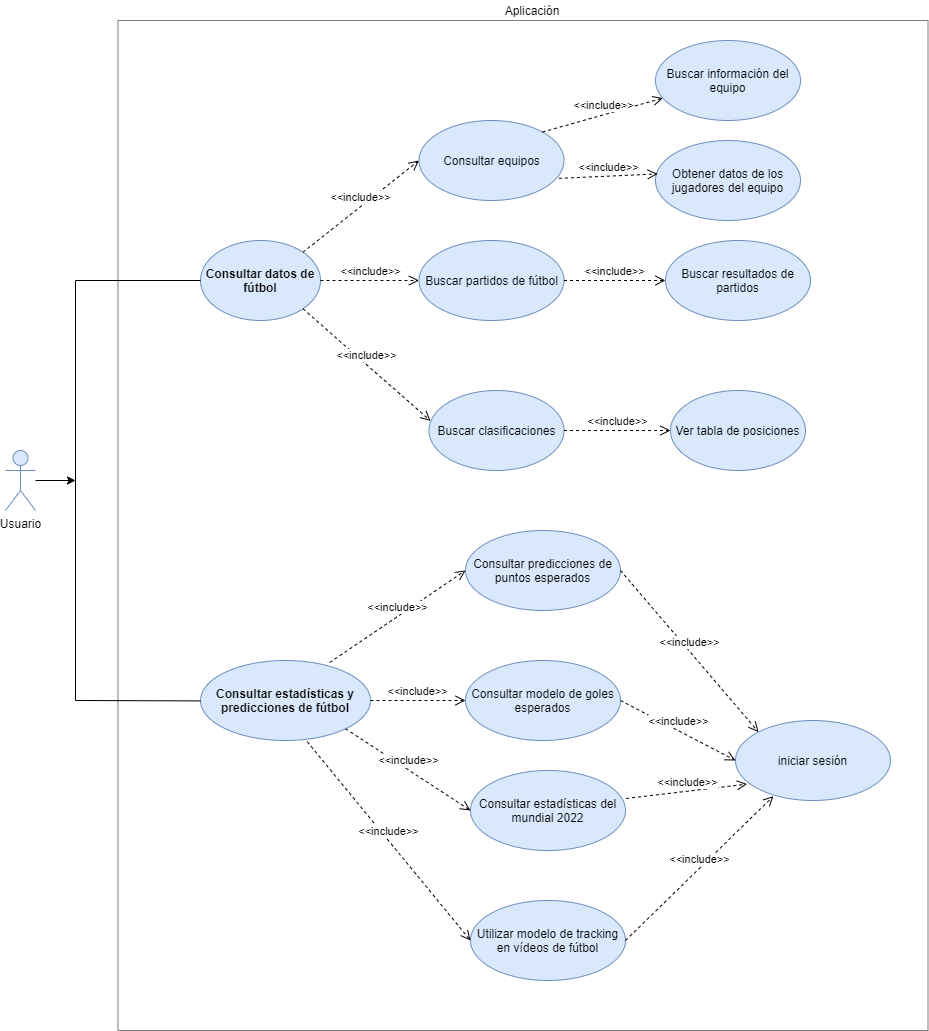
\includegraphics[width=1\linewidth]{img/casoDeUso.png}
    \caption{Diagrama de casos de uso}
    \label{fig:enter-label}
\end{figure}

\subsection{Actores}
El único actor que se contempla en los casos de uso se corresponderá con la figura del usuario.

\begin{table}[h!]
    \centering
    \begin{tabularx}{\linewidth}{ p{0.21\columnwidth} p{0.71\columnwidth} }
        \toprule
        \textbf{CU-1}    & \textbf{Consultar datos de fútbol}\\
        \toprule
        \textbf{Versión}              & 1.0    \\
        \textbf{Autor}                & Miguel Ángel Extremo Cabornero \\
        \textbf{Requisitos asociados} & RF-1 \\
        \textbf{Descripción}          & El usuario puede consultar datos sobre partidos, equipos y clasificaciones. \\
        \textbf{Precondición}         & El usuario debe tener acceso a la aplicación. \\
        \textbf{Acciones}             &
        \begin{enumerate}
            \item El usuario selecciona una de las opciones para consultar datos de fútbol.
            \item El sistema muestra opciones para consultar datos sobre partidos, equipos y clasificaciones.
        \end{enumerate}\\
        \textbf{Postcondición}        & El usuario obtiene la información solicitada. \\
        \textbf{Excepciones}          & Error en la conexión con la API. \\
        \textbf{Importancia}          & Alta \\
        \bottomrule
    \end{tabularx}
    \caption{CU-1 Consultar datos de fútbol.}
\end{table}


\begin{table}[p]
    \centering
    \begin{tabularx}{\linewidth}{ p{0.21\columnwidth} p{0.71\columnwidth} }
        \toprule
        \textbf{CU-1.1}    & \textbf{Consultar equipos}\\
        \toprule
        \textbf{Versión}              & 1.0    \\
        \textbf{Autor}                & Miguel Ángel Extremo Cabornero \\
        \textbf{Requisitos asociados} & RF-1.1 \\
        \textbf{Descripción}          & El usuario puede consultar información detallada de los equipos de fútbol. \\
        \textbf{Precondición}         & El usuario debe tener acceso a la aplicación. \\
        \textbf{Acciones}             &
        \begin{enumerate}
            \item El usuario selecciona la opción de consultar equipos.
            \item El usuario introduce el nombre de un equipo.
            \item El sistema muestra la información del equipo introducido por el usuario.
        \end{enumerate}\\
        \textbf{Postcondición}        & El usuario visualiza la información del equipo seleccionado. \\
        \textbf{Excepciones}          & 
        \begin{enumerate}
            \item El equipo seleccionado no tiene información disponible.
            \item Error en la conexión con la API.
        \end{enumerate}\\
        \textbf{Importancia}          & Alta \\
        \bottomrule
    \end{tabularx}
    \caption{CU-1.1 Consultar equipos.}
\end{table}


\begin{table}[p]
    \centering
    \begin{tabularx}{\linewidth}{ p{0.21\columnwidth} p{0.71\columnwidth} }
        \toprule
        \textbf{CU-1.1.1}    & \textbf{Obtener datos de los jugadores del equipo}\\
        \toprule
        \textbf{Versión}              & 1.0    \\
        \textbf{Autor}                & Miguel Ángel Extremo Cabornero \\
        \textbf{Requisitos asociados} & RF-1.1.2 \\
        \textbf{Descripción}          & La aplicación muestra información de los jugadores del equipo seleccionado. \\
        \textbf{Precondición}         & El usuario debe haber seleccionado un equipo. \\
        \textbf{Acciones}             &
        \begin{enumerate}
            \item El usuario selecciona un equipo.
            \item El sistema muestra la lista de jugadores del equipo.
        \end{enumerate}\\
        \textbf{Postcondición}        & El usuario visualiza la lista de jugadores y su información. \\
        \textbf{Excepciones}          & Información no disponible para los jugadores del equipo. \\
        \textbf{Importancia}          & Media \\
        \bottomrule
    \end{tabularx}
    \caption{CU-1.1.1 Obtener datos de los jugadores del equipo.}
\end{table}

\begin{table}[p]
    \centering
    \begin{tabularx}{\linewidth}{ p{0.21\columnwidth} p{0.71\columnwidth} }
        \toprule
        \textbf{CU-1.2}    & \textbf{Buscar partidos de fútbol}\\
        \toprule
        \textbf{Versión}              & 1.0    \\
        \textbf{Autor}                & Miguel Ángel Extremo Cabornero \\
        \textbf{Requisitos asociados} & RF-1.2 \\
        \textbf{Descripción}          & El usuario puede buscar información sobre partidos de fútbol. \\
        \textbf{Precondición}         & El usuario debe tener acceso a la aplicación. \\
        \textbf{Acciones}             &
        \begin{enumerate}
            \item El usuario selecciona la opción de buscar partidos de fútbol.
            \item El sistema muestra un formulario de búsqueda de partidos.
            \item El usuario ingresa los criterios de búsqueda y envía el formulario.
            \item El sistema muestra los resultados de la búsqueda.
        \end{enumerate}\\
        \textbf{Postcondición}        & El usuario visualiza los partidos de fútbol que coinciden con los criterios de búsqueda. \\
        \textbf{Excepciones}          & No se encuentran partidos que coincidan con los criterios de búsqueda. \\
        \textbf{Importancia}          & Alta \\
        \bottomrule
    \end{tabularx}
    \caption{CU-1.2 Buscar partidos de fútbol.}
\end{table}


\begin{table}[p]
    \centering
    \begin{tabularx}{\linewidth}{ p{0.21\columnwidth} p{0.71\columnwidth} }
        \toprule
        \textbf{CU-1.3}    & \textbf{Buscar clasificaciones}\\
        \toprule
        \textbf{Versión}              & 1.0    \\
        \textbf{Autor}                & Miguel Ángel Extremo Cabornero \\
        \textbf{Requisitos asociados} & RF-1.3 \\
        \textbf{Descripción}          & El usuario puede buscar clasificaciones de fútbol. \\
        \textbf{Precondición}         & El usuario debe tener acceso a la aplicación. \\
        \textbf{Acciones}             &
        \begin{enumerate}
            \item El usuario selecciona la opción de buscar clasificaciones.
            \item El usuario comienza a escribir el nombre de una liga.
            \item El sistema muestra sugerencias de ligas al usuario.
        \end{enumerate}\\
        \textbf{Postcondición}        & El usuario visualiza la clasificación de la liga. \\
        \textbf{Excepciones}          & No se encuentran clasificaciones disponibles. \\
        \textbf{Importancia}          & Alta \\
        \bottomrule
    \end{tabularx}
    \caption{CU-1.3 Buscar clasificaciones.}
\end{table}

\begin{table}[p]
    \centering
    \begin{tabularx}{\linewidth}{ p{0.21\columnwidth} p{0.71\columnwidth} }
        \toprule
        \textbf{CU-2}    & \textbf{Consultar estadísticas y predicciones de fútbol}\\
        \toprule
        \textbf{Versión}              & 1.0    \\
        \textbf{Autor}                & Miguel Ángel Extremo Cabornero \\
        \textbf{Requisitos asociados} & RF-2 \\
        \textbf{Descripción}          & El usuario puede consultar estadísticas y predicciones de fútbol, incluyendo puntos esperados, modelo de goles esperados y estadísticas del Mundial 2022. \\
        \textbf{Precondición}         & El usuario debe tener acceso a la aplicación y haber iniciado sesión. \\
        \textbf{Acciones}             &
        \begin{enumerate}
            \item El usuario selecciona la opción de consultar estadísticas y predicciones.
            \item El sistema muestra opciones para consultar puntos esperados, modelo de goles esperados y estadísticas del Mundial 2022.
        \end{enumerate}\\
        \textbf{Postcondición}        & El usuario obtiene las estadísticas y predicciones solicitadas. \\
        \textbf{Excepciones}          & Error en la conexión con la API. \\
        \textbf{Importancia}          & Alta \\
        \bottomrule
    \end{tabularx}
    \caption{CU-2 Consultar estadísticas y predicciones de fútbol.}
\end{table}


\begin{table}[p]
    \centering
    \begin{tabularx}{\linewidth}{ p{0.21\columnwidth} p{0.71\columnwidth} }
        \toprule
        \textbf{CU-2.1}    & \textbf{Consultar predicciones de puntos esperados}\\
        \toprule
        \textbf{Versión}              & 1.0    \\
        \textbf{Autor}                & Miguel Ángel Extremo Cabornero \\
        \textbf{Requisitos asociados} & RF-2.1 \\
        \textbf{Descripción}          & El usuario puede consultar predicciones de puntos esperados para los equipos de fútbol. \\
        \textbf{Precondición}         & El usuario debe tener acceso a la aplicación y haber iniciado sesión. \\
        \textbf{Acciones}             &
        \begin{enumerate}
            \item El usuario selecciona la opción de consultar predicciones de puntos esperados.
            \item El sistema muestra las predicciones de puntos esperados para las ligas.
            \item El sistema muestra un gráfico de la posición de los equipos en cada jornada.
        \end{enumerate}\\
        \textbf{Postcondición}        & El usuario visualiza las predicciones de puntos esperados. \\
        \textbf{Excepciones}          & No se encuentran predicciones disponibles. \\
        \textbf{Importancia}          & Alta \\
        \bottomrule
    \end{tabularx}
    \caption{CU-2.1 Consultar predicciones de puntos esperados.}
\end{table}


\begin{table}[p]
    \centering
    \begin{tabularx}{\linewidth}{ p{0.21\columnwidth} p{0.71\columnwidth} }
        \toprule
        \textbf{CU-2.2}    & \textbf{Consultar modelo de goles esperados}\\
        \toprule
        \textbf{Versión}              & 1.0    \\
        \textbf{Autor}                & Miguel Ángel Extremo Cabornero \\
        \textbf{Requisitos asociados} & RF-2.2 \\
        \textbf{Descripción}          & El usuario puede consultar el modelo de goles esperados. \\
        \textbf{Precondición}         & El usuario debe tener acceso a la aplicación y haber iniciado sesión. \\
        \textbf{Acciones}             &
        \begin{enumerate}
            \item El usuario selecciona la opción de consultar modelo de goles esperados.
            \item El sistema muestra el modelo de goles esperados..
        \end{enumerate}\\
        \textbf{Postcondición}        & El usuario visualiza el modelo de goles esperados. \\
        \textbf{Excepciones}          & No se encuentra el modelo de goles esperados. \\
        \textbf{Importancia}          & Alta \\
        \bottomrule
    \end{tabularx}
    \caption{CU-2.2 Consultar modelo de goles esperados.}
\end{table}


\begin{table}[p]
    \centering
    \begin{tabularx}{\linewidth}{ p{0.21\columnwidth} p{0.71\columnwidth} }
        \toprule
        \textbf{CU-2.3}    & \textbf{Consultar estadísticas del Mundial 2022}\\
        \toprule
        \textbf{Versión}              & 1.0    \\
        \textbf{Autor}                & Miguel Ángel Extremo Cabornero \\
        \textbf{Requisitos asociados} & RF-2.3 \\
        \textbf{Descripción}          & El usuario puede consultar estadísticas del Mundial 2022. \\
        \textbf{Precondición}         & El usuario debe tener acceso a la aplicación y haber iniciado sesión. \\
        \textbf{Acciones}             &
        \begin{enumerate}
            \item El usuario selecciona la opción de consultar estadísticas del Mundial 2022.
            \item El sistema muestra las estadísticas del Mundial 2022.
            \item El usuario puede elegir de que jugador quiere visualizar el gráfico de estadísticas del Mundial 2022.
            \item El usuario puede comprender los gráficos fácilmente.
        \end{enumerate}\\
        \textbf{Postcondición}        & El usuario visualiza las estadísticas del Mundial 2022. \\
        \textbf{Excepciones}          & No se encuentran estadísticas disponibles. \\
        \textbf{Importancia}          & Media \\
        \bottomrule
    \end{tabularx}
    \caption{CU-2.3 Consultar estadísticas del Mundial 2022.}
\end{table}


\begin{table}[p]
    \centering
    \begin{tabularx}{\linewidth}{ p{0.21\columnwidth} p{0.71\columnwidth} }
        \toprule
        \textbf{CU-2.4}    & \textbf{Utilizar modelo de tracking en vídeos de fútbol}\\
        \toprule
        \textbf{Versión}              & 1.0    \\
        \textbf{Autor}                & Miguel Ángel Extremo Cabornero \\
        \textbf{Requisitos asociados} & RF-2.4 \\
        \textbf{Descripción}          & El usuario puede utilizar el modelo de tracking en vídeos de fútbol. \\
        \textbf{Precondición}         & El usuario debe tener acceso a la aplicación y haber iniciado sesión. \\
        \textbf{Acciones}             &
        \begin{enumerate}
            \item El usuario selecciona la opción de utilizar modelo de tracking (ImageAI).
            \item El sistema solicita al usuario que cargue un vídeo de fútbol.
            \item El usuario carga el vídeo.
            \item El sistema procesa el vídeo utilizando el modelo de ImageAI.
            \item El sistema muestra el vídeo procesado al usuario.
        \end{enumerate}\\
        \textbf{Postcondición}        & El usuario visualiza el vídeo con el tracking aplicado. \\
        \textbf{Excepciones}          & Error en el procesamiento del vídeo. \\
        \textbf{Importancia}          & Alta \\
        \bottomrule
    \end{tabularx}
    \caption{CU-2.4 Utilizar modelo de tracking en vídeos de fútbol.}
\end{table}


\begin{table}[p]
    \centering
    \begin{tabularx}{\linewidth}{ p{0.21\columnwidth} p{0.71\columnwidth} }
        \toprule
        \textbf{CU-3}    & \textbf{Autenticación}\\
        \toprule
        \textbf{Versión}              & 1.0    \\
        \textbf{Autor}                & Miguel Ángel Extremo Cabornero \\
        \textbf{Requisitos asociados} & RF-3 \\
        \textbf{Descripción}          & El usuario puede iniciar sesión en la aplicación. \\
        \textbf{Precondición}         & El usuario debe tener una cuenta de Google y acceso a la aplicación. \\
        \textbf{Acciones}             &
        \begin{enumerate}
            \item El usuario selecciona la opción de iniciar sesión.
            \item El sistema muestra un botón de inicio de sesión.
            \item El usuario inicia sesión con su cuenta de Google.
            \item El sistema verifica que la cuenta es correcta e inicia sesión.
        \end{enumerate}\\
        \textbf{Postcondición}        & El usuario está autenticado y puede acceder a funcionalidades protegidas. \\
        \textbf{Excepciones}          & Credenciales incorrectas o error en la autenticación. \\
        \textbf{Importancia}          & Alta \\
        \bottomrule
    \end{tabularx}
    \caption{CU-3 Autenticación.}
\end{table}

